\section{Análisis de diferentes soluciones propuestas}
Vamos a proponer dos escenarios posibles para poder analizar sus soluciones. Estos dos escenarios son de la forma: 
 %insertar imagen!!!


Primero analizamos el primer caso de 3 días ya que es el proporcionado por la cátedra.

$$
n = 3,\ \ S=(1, 5, 4),\ \ E=(10,2,2)
$$

En este
notamos que la ganancia de un día $i$ puede tomar 2 valores posibles: 
\begin{itemize}
    \item Suma entre la ganancia del día anterior y $min(e_i, s_d)$, con $d$ cantidad de días seguidos entrenando
    \item Suma entre la ganancia de dos días antes y $min(e_i, s_1)$
\end{itemize}

Esto debido a que observamos una relación con el problema planteado de Juan el Vago, en el que buscábamos la mayor ganancia,
pero sin trabajar dos días seguidos.

Para esta instancia, supusimos erroneamente, que la ganancia máxima para un día $i$ iba a estar dada si en cada día de entrenamiento 
se maximizaba su ganancia. De esta forma, cada vez que se necesite la ganancia máxima de un día o más anteriores, esta ya iba a estar calculada
anteriormente. Para poder calcular esta propuesta propusimos el siguiente algoritmo:
$g(i, d)= max{g(n-1) + min(e_i,s_d), g(n-2) + min(e_i,s_1)}$ , 

De esta manera, este algoritmo daba la respuesta esperada que es 7 en el primer caso de 3 días.

El inconveniente en este algortimo es que al querer maximizar cada día solo comparando si el día anterior hubiera convenido
descansar o no, no se tiene en consideración el hecho de que hay escenarios donde el descanso es conveniente en un día
$j < i-1$ y solo se hace evidente en el día $i$. 
Esto se debe a que la ganancia máxima en un $i$-ésimo día es esencialmente la suma del mínimo entre el esfuerzo requerido y la 
energía disponible.

Dado que esta ganancia está condicionada por los niveles de energía de cada día, en ocasiones es más 
conveniente que la ganancia relativa de un día no sea óptima individualmente, sino que en conjunto 
ofrezca la mayor ganancia total. El algoritmo propuesto no aborda adecuadamente esta complejidad, 
ya que solo considera esta condición con respecto a los dos días anteriores, lo que limita la 
capacidad de adaptación a situaciones donde la estrategia de descanso óptima se extiende en un 
período más largo.

Al darnos cuenta de este problema, procedimos a utilizar una planilla de cálculo para ayudarnos a resolverlo.
Arreglamos $E$ verticalmente y $S$ horizontalmente en un cuadro de doble entrada. Luego, cada
casilla $(i, j)$ era la ganancia parcial que podríamos obtener si ese fuera el $i$-ésimo día
de entrenamiento consecutivo para el día $j$ del plan de entrenamiento. Notamos que la ganancia
máxima hasta el entrenamiento $j$ era el máximo de las ganancias parciales de la misma fila.
Decidimos entonces colocar a la izquierda una columna auxiliar que contenía la ganancia maxima
de la fila inferior. Ver resultado en la figura \ref{fig:planilla_caso_2}.

\begin{figure}[H]
    \centering
    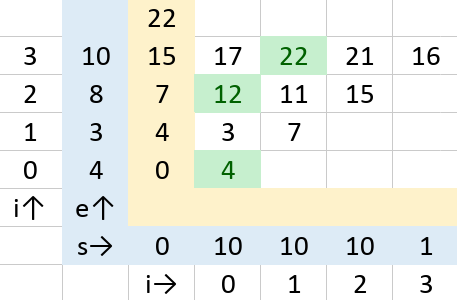
\includegraphics[width=0.5\textwidth]{img/planilla_caso_2.png}
    \caption{Caso 2 planilla}
    \label{fig:planilla_caso_2}
\end{figure}

Luego, logramos abstraer las funciones, mostradas en la figuras \ref{fig:planilla_completa},
\ref{fig:formulas_planilla_1} y  \ref{fig:formulas_planilla_2}.

\begin{figure}[ht]
    \centering
    \begin{minipage}[b]{0.495\textwidth}
        \centering
        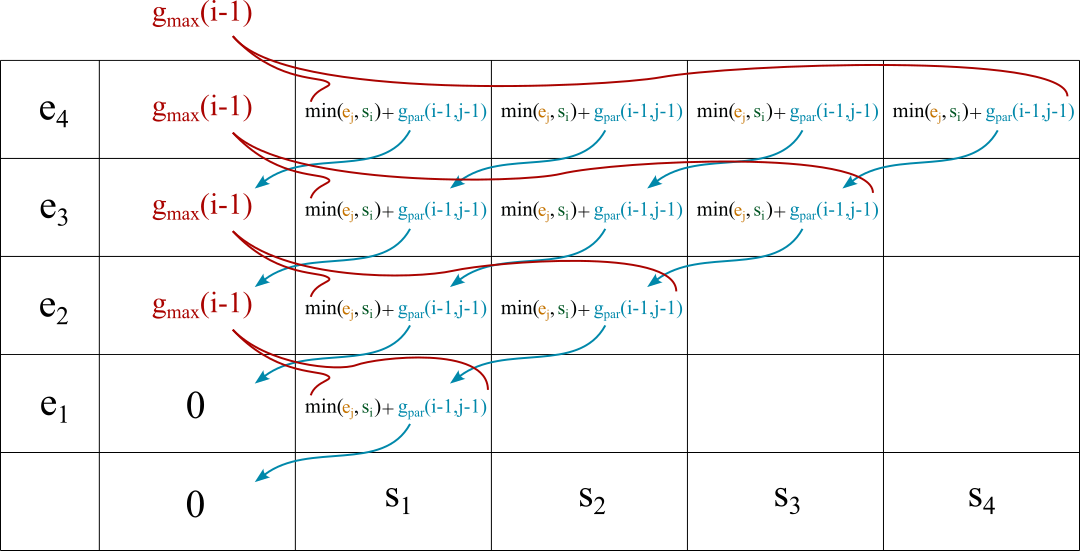
\includegraphics[width=\textwidth]{img/formulas_planilla_1.png}
        \label{fig:formulas_planilla_1}
    \end{minipage}
    \begin{minipage}[b]{0.495\textwidth}
        \centering
        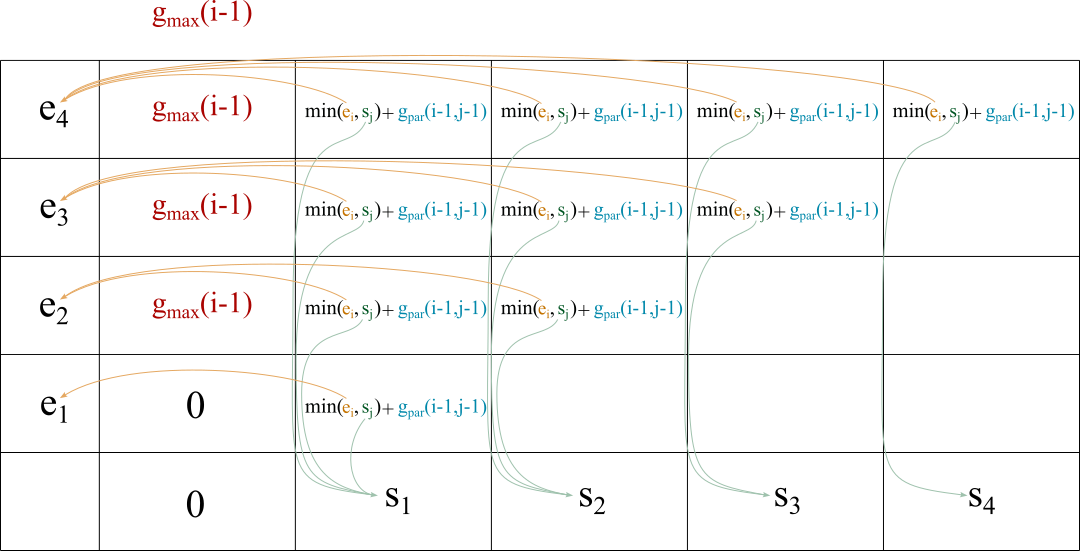
\includegraphics[width=\textwidth]{img/formulas_planilla_2.png}
        \label{fig:formulas_planilla_2}
    \end{minipage}
\end{figure}

\begin{figure}[H]
    \centering
    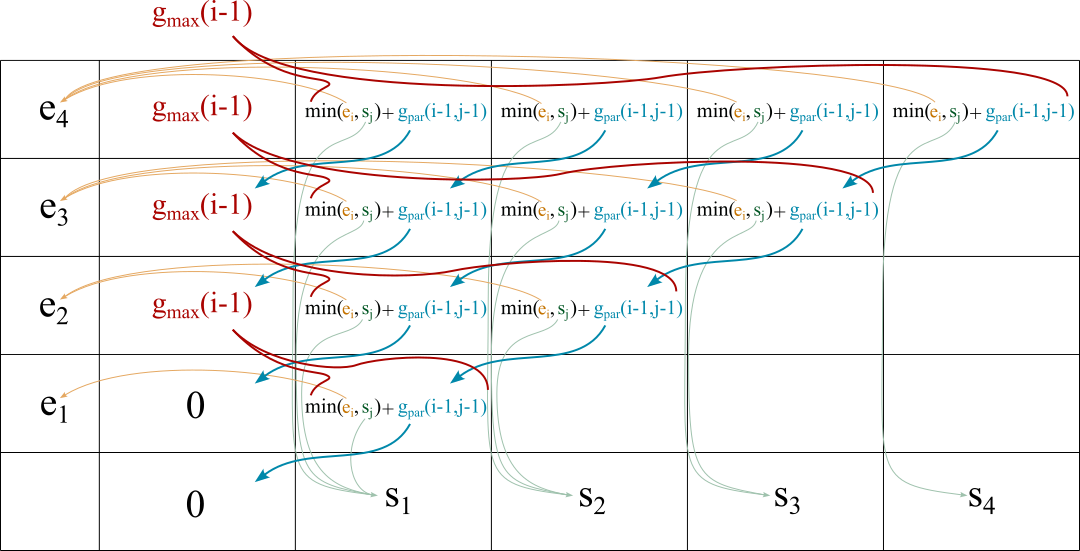
\includegraphics[width=1\textwidth]{img/planilla_completa.png}
    \caption{Formulas en planilla}
    \label{fig:planilla_completa}
\end{figure}


El algoritmo presentado tiene una complejidad temporal de $\operatorname{O}(n^2)$.
Esto se debe a que, para obtener la solución óptima, requerimos analizar cada día de entrenamiento, con todas sus
variantes de energía disponible por día.\
Técnicamente lo que hacemos es recorrer una matriz de $n*n$, siendo n la cantidad de días a entrenar (igual cantidad que
los valores que toman las energías).\
Ahora, para cada día, calculamos el ganancia parcial respecto a los días anteriores, es decir,



\section{Posibles algoritmos}

Posterior a nuestro análisis, propusimos dos algoritmos:

\subsection{Ordenando por $a_i$ de forma creciente}
Este algorítmo sigue las siguientes indicaciones:
\begin{itemize}
    \item Ordenar los compilados de menor a mayor tiempo de análisis por parte de los ayudantes.
    \item Cada vez que termina Scaloni de ver un compilado, inmediatamente un ayudante es asignado a visualizarlo.
\end{itemize}

\subsection{Ordenando por $a_i$ de forma decreciente}
Este algoritmo sigue las siguientes indicaciones:
\begin{itemize}
    \item Ordenar los compilados de mayor a menor tiempo de análisis por parte de los ayudantes.
    \item Cada vez que termina Scaloni de ver un compilado, inmediatamente un ayudante es asignado a visualizarlo.
\end{itemize}

Comparemos cómo se desempeñan nuestros dos algorítmos en cada escenario propuesto:

\subsection{Resultados obtenidos del Caso 1}

% \begin{figure}[H]
%     \centering
%     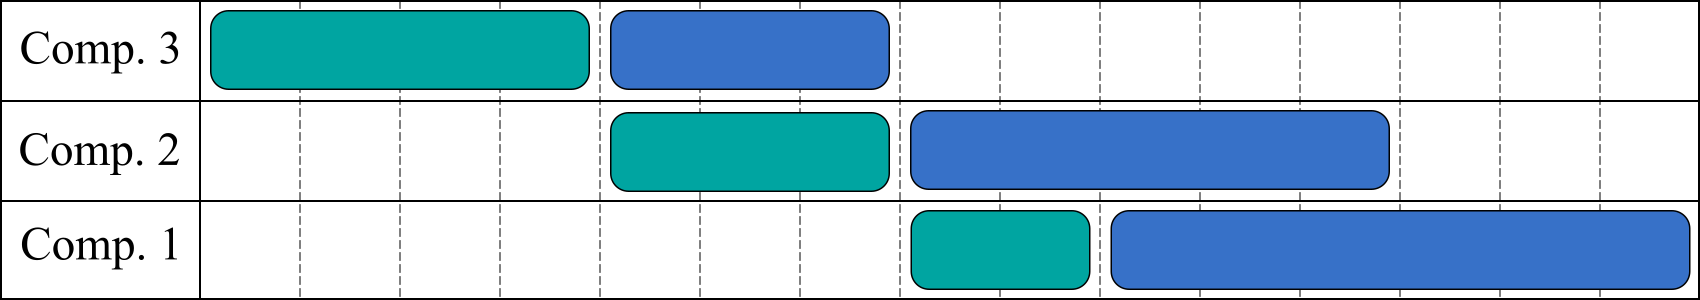
\includegraphics[width=1\textwidth]{img/caso-1-creciente.png}
%     \caption{Caso 1 ordenado de forma creciente por $a_i$}
%     \label{fig:Caso 1 ordenado de forma creciente por $a_i$}
% \end{figure}

% \begin{figure}[H]
%     \centering
%     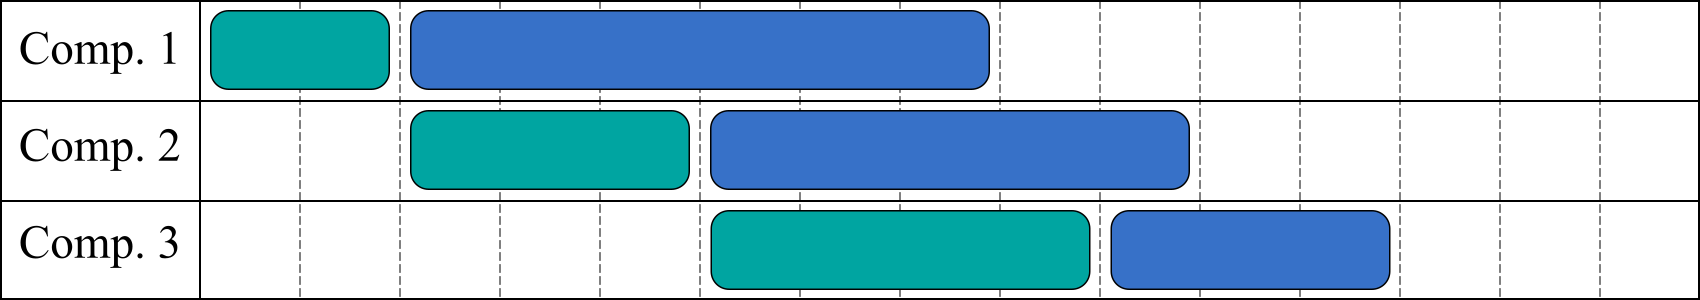
\includegraphics[width=1\textwidth]{img/caso-1-decreciente.png}
%     \caption{Caso 1 ordenado de forma decreciente por $a_i$}
%     \label{fig:Caso 1 ordenado de forma decreciente por $a_i$}
% \end{figure}


\subsection{Resultados obtenidos del Caso 2}

% \begin{figure}[H]
%     \centering
%     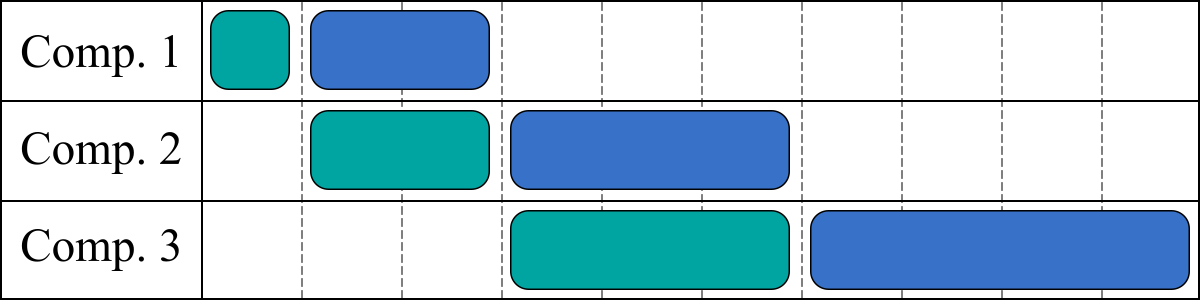
\includegraphics[width=1\textwidth]{img/caso-2-creciente.png}
%     \caption{Caso 2 ordenado de forma creciente por $a_i$}
%     \label{fig:Caso 2 ordenado de forma creciente por $a_i$}
% \end{figure}

% \begin{figure}[H]
%     \centering
%     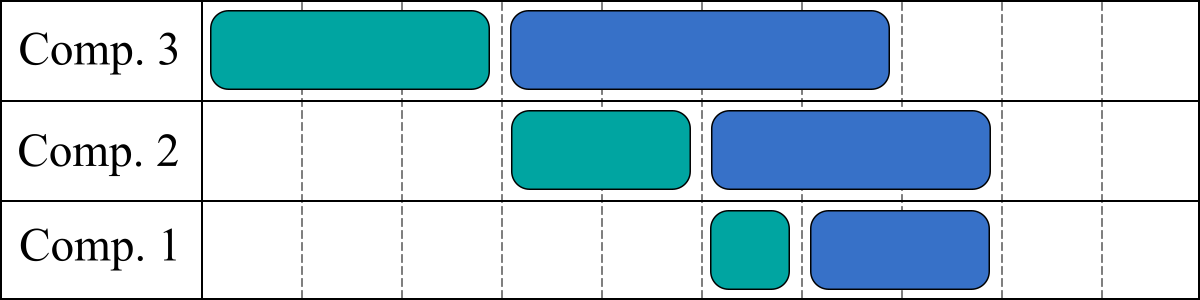
\includegraphics[width=1\textwidth]{img/caso-2-decreciente.png}
%     \caption{Caso 2 ordenado de forma decreciente por $a_i$}
%     \label{fig:Caso 2 ordenado de forma decreciente por $a_i$}
% \end{figure}

Como se puede observar, para ambos casos el ordenamiento decreciente resulta en un tiempo total menor.

\section{Demostración}

Procederemos a demostrar que ordenar los compilados por $a_i$ de forma decreciente minimiza el tiempo total.

Llamamos $C$ al conjunto ordenado de $n$ compilados, $s_i$ el tiempo que le tardar visualizar a Scaloni el $i$-ésimo compilado, y
$a_i$ lo que le tarda a un ayudante. Además, al tiempo que tarda Scaloni analizar los compilados hasta el $k$-ésimo lo representaremos como $S_k$.

$$
S_{k}=\sum_{i=1}^{k}s_{i} 
$$

Luego, el tiempo total que se tarda en analizar los compilados hasta el $k$-ésimo, en el orden
en el que se los presenta, sigue la siguiente formula:


$$
T_{k} = \begin{cases}
s_{1}+a_{1} & k=1 \\
\displaystyle\max{(T_{k-1},S_{k}+a_{k})} & k>1
\end{cases}
$$

Ordenar $C$ para minimizar $T_{n}$ requiere minimizar $\max{(T_{n-1},S_{n}+a_{n})}$. Como $S_{n}$ es independiente del orden de $C$, $S_{n}+a_{n}$ se minimiza colocando último al compilado con el tiempo del ayudante más pequeño. Luego, $T_{n-1}$ se minimiza de la misma manera, resultando en un algoritmo recursivo. Solo nos falta justificar por qué el orden que minimiza $S_{n}+a_{n}$ también minimiza $\max{(T_{n-1},S_{n}+a_{n})}$. Haremos esto partiendo de la asumpción de que se respeta el orden propuesto y de que modificarlo resulta en un $T_n$ más grande.

\begin{itemize}

    \item Si $\max{(T_{n-1},S_{n}+a_{n})} = S_{n}+a_{n}$ ($\implies S_{n}+a_{n} \geq T_{n-1}$)

    Es el caso más trivial, ya que minimizar $S_{n}+a_{n}$ también minimiza $\max{(T_{n-1},S_{n}+a_{n})}$.

    \item Si $\max{(T_{n-1},S_{n}+a_{n})} = T_{n-1}$ ($\implies T_{n-1} \geq S_{n}+a_{n}$)

    Este caso implica que existe un compilado $j$ tal que $a_{j} \geq \sum^{n}_{i=j+1}s_{i}+a_{n} \implies a_{j} > a_{n}$.
    Colocar a este compilado último causaría que $T_{n}'= S_{n}+a_{j}$, y

\end{itemize}

$$
T_{n}' = S_{n}+a_{j}, \ \ \ \  T_{n} = S_{j}+a_{j} 
$$

$$
\begin{aligned}
S_{n} & > S_{j} \\
S_{n} + a_{j}  & > S_{n} + a_{j}  \\
T_{n}' & > T_{n}
\end{aligned}
$$

Esto demuestra que el orden de $C$ que minimiza $T_n$ es con los tiempos $a_i$ decrecientes.


% \begin{figure}[H]
%     \centering
%     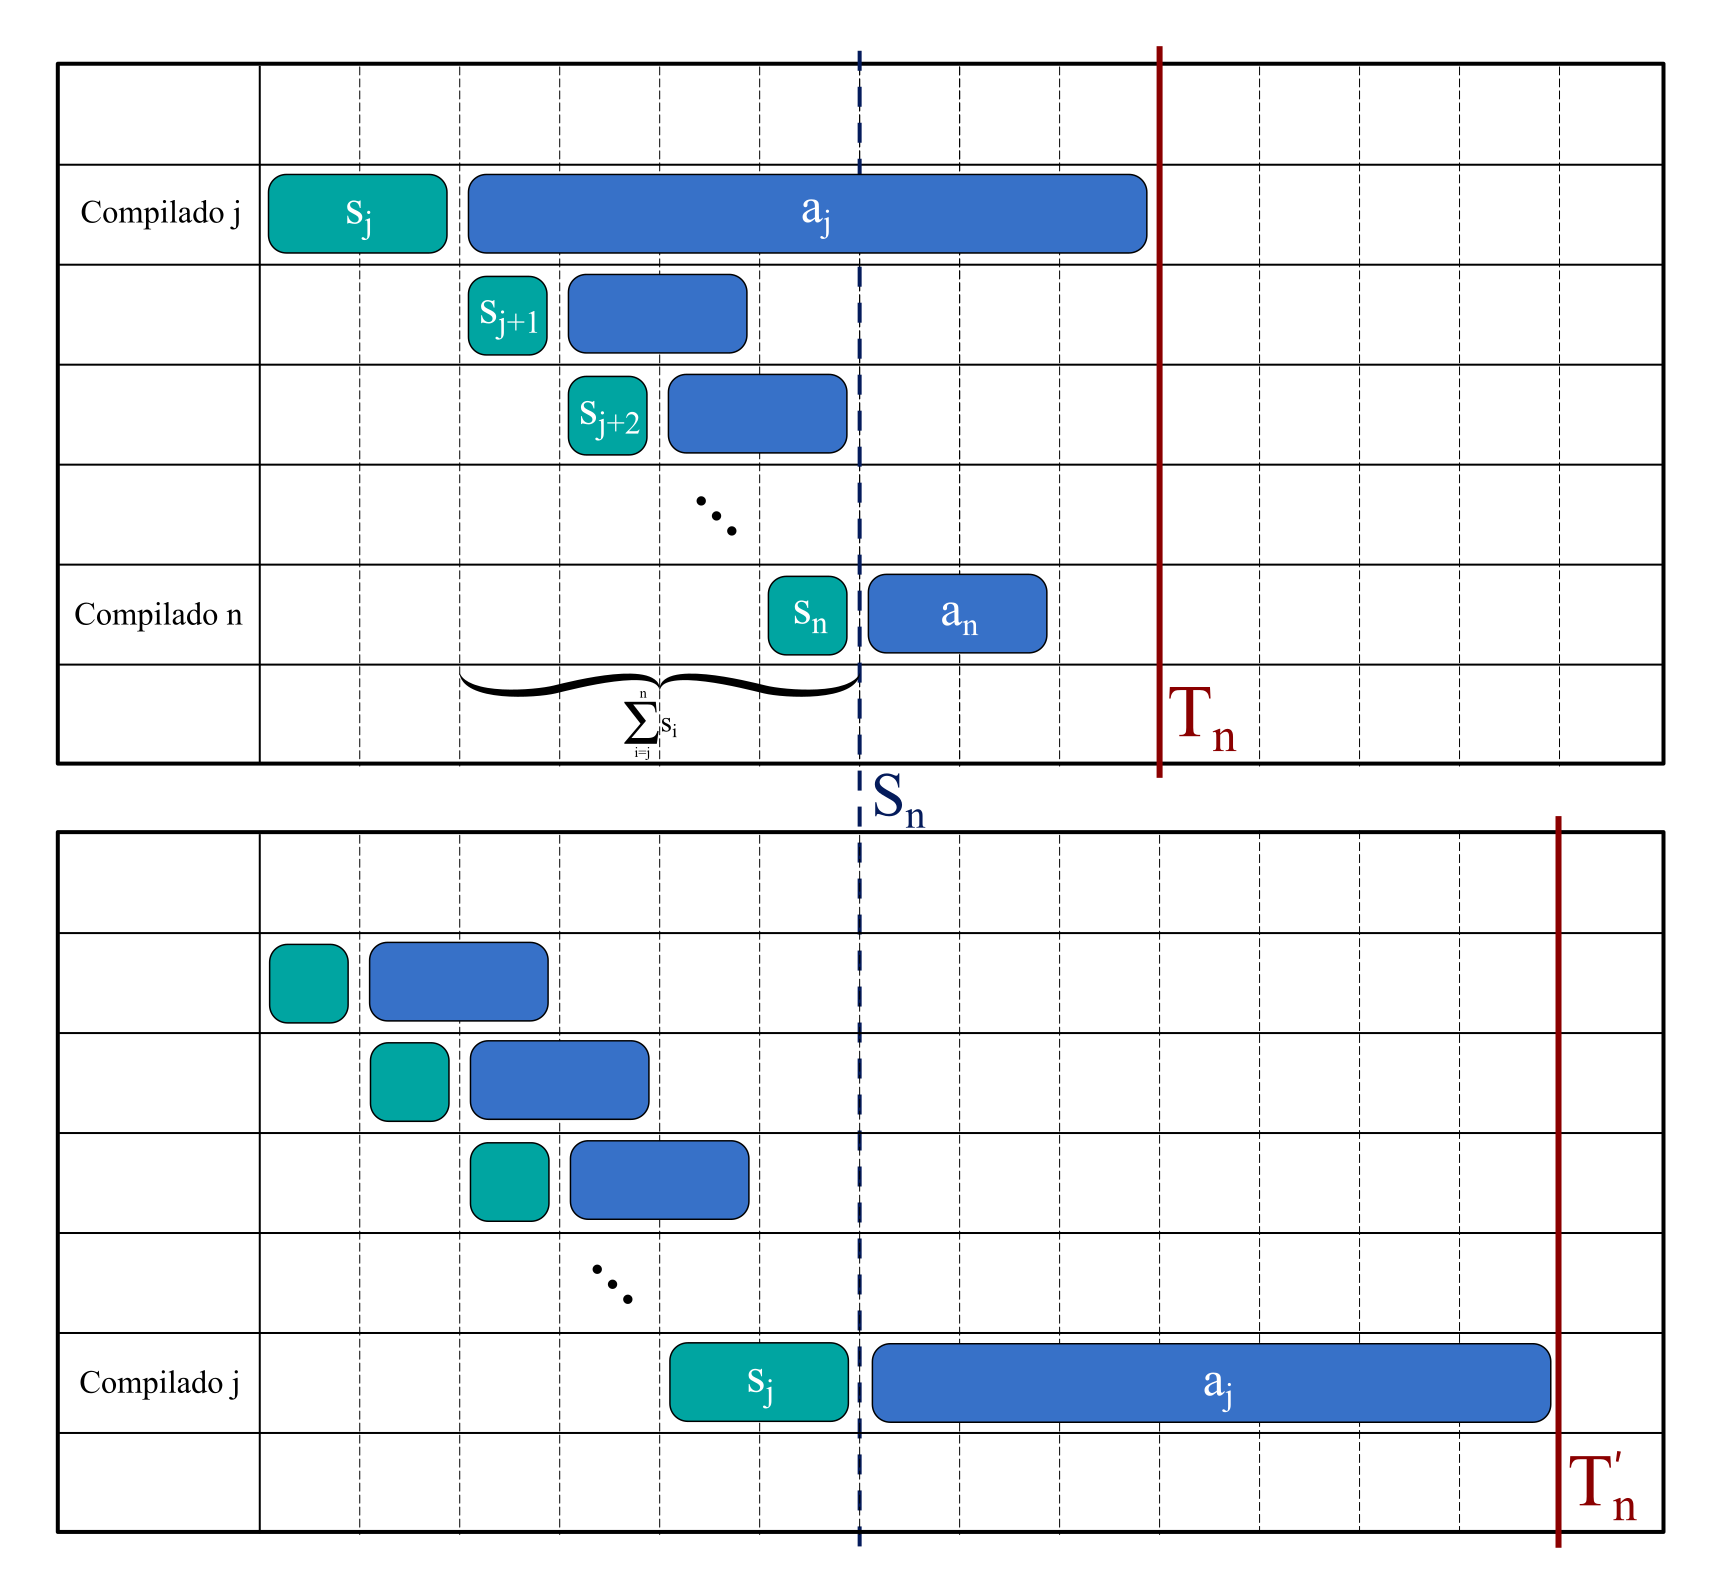
\includegraphics[width=1\textwidth]{img/demostracion.png}
%     \caption{Ilustración de la demostración}
%     \label{fig:Ilustración de la demostración}
% \end{figure}


\textbf{Para ello propusimos el siguiente algoritmo:}

En primer lugar, hemos definido una clase llamada \texttt{Compilado} para modelar el compilado de cada 
oponente, con los atributos \texttt{tiempo\_scaloni} y \texttt{tiempo\_ayudante}, que almacenan 
el tiempo que le lleva analizarlo a Scaloni y a algún ayudante, respectivamente.

\begin{lstlisting}[language=Python]
class Compilado:
    def __init__(self, scaloni, ayudante):
        self.tiempo_scaloni = scaloni
        self.tiempo_ayudante = ayudante
\end{lstlisting}

De esta forma, y teniendo en cuenta los criterios previamente detallados, definimos la función
\texttt{compilados\_ordenados\_de\_forma\_optima} que recibe como parámetro un arreglo con
elementos de la clase \texttt{Compilado}. Esta ordena el arreglo en función del tiempo requerido
por los asistentes para visualizar cada compilado, en orden descendente. 

\begin{lstlisting}[language=Python]
def compilados_ordenados_de_forma_optima(compilados):
    return sorted(compilados, key=lambda compilado: compilado.tiempo_ayudante, reverse=True)
\end{lstlisting}



\begin{itemize}
    \item Los asistentes realizan el análisis de cada uno de los compilados asignados en paralelo. Por lo 
tanto, el tiempo que se invierte en la revisión de un compilado específico de máxima duración, 
puede ser aprovechado de manera tal que este sea visto mientras Scaloni se dedica a la revisión
de otros compilados. De esta forma, nos aseguramos que se minimice el tiempo que suman los ayudantes 
en la resvisión total. 
    \item También en esta solución tiene en consideración el análisis 2 descripto previamente, ya que en el mejor de los casos,
    la $\sum_{k=1}^{n} s_k + a_n$ termina siendo la mínima ya que, por la forma del ordenamiento del algorítmo, $a_n$ es la duración del compilado más corto.

\end{itemize}